\section{\lr{Out of order execution}}
\link{https://en.wikipedia.org/wiki/Tomasulo\%27s\_algorithm}{منبع}
\begin{enumerate}
    \item به صورت خلاصه این الگوریتم برای هر \lr{execution unit} چندین \lr{flag}
    نگه می‌دارد. به این جدول
    \lr{reservation status}
    گفته می‌شود. مثلا در عکس
    \ref{pic:reservation_status}
    سه واحد جمع کننده و دو واحد ضرب کننده داریم.
    \begin{figure}[H]
        \centering
        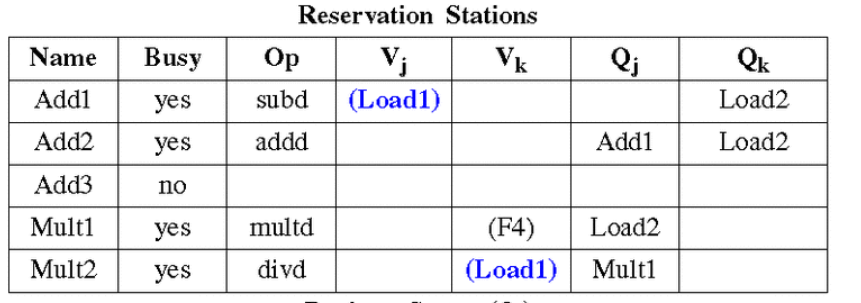
\includegraphics[scale=0.5]{pics/5-reservation-status.png}
        \caption{\lr{Reservation Status}}
        \label{pic:reservation_status}
    \end{figure}
    مرحله‌ی اول برای دستورات
    \lr{issue}
    هست. در این مرحله عملا ما دستور را به یکی از واحد‌های اجرایی
    \lr{CPU}
    می‌دهیم. به عنوان مثال اگر درخواست ضرب شده بود و یک واحد ضرب کننده خالی بود، به واحد ضرب کننده
    دستور را
    \emph{issue}
    می‌کنیم. اما در صورتی که واحد ضرب کننده‌ای خالی نبود باید اینقدر دستور را نگه داریم که یکی
    خالی شود.
    اما مشکل دیگری که می‌تواند به وجود آید این است که عملگر‌های دستور آماده نباشند. مثلا یک دستور
    \codeword{add}
    باید منتظر جواب یک دستور
    \codeword{mult}
    بماند. در این حالت باز نیست دستور را
    \lr{issue}
    می‌کنیم ولی از آنجا که مقدار واقعی رجیستر را نداریم،‌ در واحد محاسباتی باید صبر کنیم که مقدار
    آن مشخص شود.

    مرحله‌ی بعدی
    \lr{execute}
    است.
\end{enumerate}